% CVPR 2022 Paper Template
% based on the CVPR template provided by Ming-Ming Cheng (https://github.com/MCG-NKU/CVPR_Template)
% modified and extended by Stefan Roth (stefan.roth@NOSPAMtu-darmstadt.de)

\documentclass[10pt,twocolumn,letterpaper]{article}

%%%%%%%%% PAPER TYPE  - PLEASE UPDATE FOR FINAL VERSION
\usepackage[final]{cvpr}      % To produce the REVIEW version
%\usepackage{cvpr}              % To produce the CAMERA-READY version
%\usepackage[pagenumbers]{cvpr} % To force page numbers, e.g. for an arXiv version

% Include other packages here, before hyperref.
\usepackage{graphicx}
\usepackage{amsmath}
\usepackage{amssymb}
\usepackage{booktabs}
%!TEX encoding = UTF-8 Unicode
\usepackage{cjk}
% uncomment this line when editing on overleaf
% \usepackage{CJKutf8}



% It is strongly recommended to use hyperref, especially for the review version.
% hyperref with option pagebackref eases the reviewers' job.
% Please disable hyperref *only* if you encounter grave issues, e.g. with the
% file validation for the camera-ready version.
%
% If you comment hyperref and then uncomment it, you should delete
% ReviewTempalte.aux before re-running LaTeX.
% (Or just hit 'q' on the first LaTeX run, let it finish, and you
%  should be clear).
\usepackage[pagebackref,breaklinks,colorlinks]{hyperref}


% Support for easy cross-referencing
\usepackage[capitalize]{cleveref}
\crefname{section}{Sec.}{Secs.}
\Crefname{section}{Section}{Sections}
\Crefname{table}{Table}{Tables}
\crefname{table}{Tab.}{Tabs.}


%%%%%%%%% PAPER ID  - PLEASE UPDATE
\def\cvprPaperID{*****} % *** Enter the CVPR Paper ID here
\def\confName{CVPR}
\def\confYear{2022}


\begin{document}
\begin{CJK}{UTF8}{bsmi}
%%%%%%%%% TITLE
\title{Predicting Future Traffic Accident Severity using A Countrywide Traffic Accident Dataset~\cite{2019arXiv190605409M}\cite{2019arXiv190909638M}}

\author{
郭立晨 \\
F94081076\\
% For a paper whose authors are all at the same institution,
% omit the following lines up until the closing ``}''.
% Additional authors and addresses can be added with ``\and'',
% just like the second author.
% To save space, use either the email address or home page, not both
\and
盧湧恩\\
F74109040\\
\and
陳均哲\\
F74109032\\
}
\maketitle

%%%%%%%%% ABSTRACT
\begin{abstract}
This paper addresses the challenge of predicting traffic accident severity, utilizing a dataset covering 1.5 million records across 49 U.S. states from 2016 to 2023. Despite challenges such as missing values and dataset imbalance, the proposed systematic framework involves statistical analysis, preprocessing, and model training. Noteworthy patterns emerge from data visualization, guiding feature reduction strategies. The experiment identifies Random Forest as the top-performing model, with f1-beta scores indicating its effectiveness in handling imbalanced datasets. Future work involves parameter tuning and incorporating external data for enhanced predictive accuracy, contributing to accident prevention and law enforcement resource optimization.
\end{abstract}

%%%%%%%%% BODY TEXT
\section{Introduction}
\label{sec:intro}

%-------------------------------------------------------------------------

\subsection{Motivation}

Traffic accidents pose significant risks to pedestrians and infrastructure, consuming a considerable amount of manpower and financial resources each year to address the issue. Therefore, through the analysis of various environmental conditions of long-term traffic accident events, including weather factors, geographical environment, traffic signals, and important infrastructure locations, we aim to predict the severity of accident base on multiple environment variables. This information can assist relevant law enforcement agencies in optimizing the allocation of labour for better deployment strategies.

\subsection{Dataset}
This dataset provides continuous records of traffic accidents covering all 49 states of the United States from February 2016 to March 2023. The data is sourced from various data providers and APIs, including traffic event data from different entities such as transportation departments, law enforcement agencies, traffic cameras, and sensors. Currently, the entire dataset contains approximately 1.5 million accident records.
The dataset includes parameters related to the severity classification of accidents, occurrence time, coordinates, city names, temperature, humidity, nearby traffic facilities, and other factors associated with accident incidents.

\subsection{Difficulty}
There are three main challenges for this experiment. First, the dataset provider mentioned difficulties with network connectivity, resulting in the inability to guarantee recording all data for every accident. Moreover, missing values will not be updated. Therefore, before using this dataset for training, a thorough examination of the data is necessary. Handling missing values for each kind of field will be a significant challenge in the preprocessing stage.
The second challenge is that the current dataset provides 47 parameters. Considering all parameters simultaneously may introduce a lot of unnecessary noise. Hence, during the training process, it's crucial to devise a method to eliminate parameters that do not significantly impact accident occurrences. The third challenge is that the dataset is highly imbalanced, accidents of severity 2 accounts nearly 80 percent of the entire dataset. Addressing such imbalanced dataset demands additional effort during model training, and evaluating models with imbalanced testing dataset necessitates careful consideration.


%------------------------------------------------------------------------

\section{System Framework}
\label{sec:formatting}

%------------------------------------------------------------------------

\subsection{Overview}
The experiment will begin with an initial statistical analysis of the dataset, including calculating the mean, median, and standard deviation. Data will also be visualized to see how it's distributed. For missing values, different imputation techniques will be utilized. To prevent biases in the training results due to extremely large or small values in numerical data, normalization and standardization will be applied. Outliers will be removed if necessary to address skewness. After data preprocessing, we intend to use Regression Analysis methods such as linear regression or logistic regression to examine the correlation between accidents and factors like weather, road conditions, and time. This allows the elimination of accident factors with weak correlations and serves as a basis for feature importance analysis. Next, the chosen accident factors will be used to train a classification model. The model’s output will categorize accident severity into four levels, ranging from minor (short delay) to severe (long delay). Finally, model performance will be evaluated using metrics such as Precision, Recall, F1 score, etc, to evaluate model performance.

\subsection{Dealing with Missing Values}
The dataset has 22 columns with missing values, including numerical and categorical data. We addressed this by dropping columns with excessive missing values and those containing irrelevant information, such as data source and destination. Four similar columns related to twilight were merged into one for simplicity. In addition, we introduced new time-related columns to enhance the dataset. One such column is "elapsed time", derived by computing the difference between starting and ending times, as we anticipated its potential significance. Moreover, we transformed the start time into six distinct columns: Year, Month, Day, Weekday, Hour, Minute. Simultaneously, the original start time and end time columns were eliminated. We organized the dataset by county and sorted it by timestamps. Numerical missing values were filled using interpolation, excluding rows without specific features within the same county beforehand. After filling numerical missing values, we simplified the wind direction column by reducing the number of classifications. Finally, rows with categorical missing values were dropped. These steps reduced the number of columns from 46 to 35 and the number of rows from 7,728,394 to 7,484,058.

\subsection{Data Visualization}
Upon conducting data visualization based on the dataset, several noteworthy patterns emerged. Notably, weather conditions categorized as Fair, Mostly Cloudy, Clear, and Cloudy were found to be the most prevalent during accidents. The data also revealed a distinct trend, with accidents of severity 2 constituting nearly 80 percent of occurrences, while accidents of severity 1 exhibited the lowest frequency. Accidents categorized as severity 4 typically entail the longer elapsed time, while those classified as severity 1 tend to have the shorter duration.
Examining the temporal aspect from 2016 to 2022, accidents of severity 2 and severity level 4 demonstrated a consistent upward trajectory, whereas severity level 3 witnessed an increase from 2016 to 2018 followed by a subsequent decline. Noteworthy variations in accident frequency were observed across months, with the highest occurrences transpiring between months 10 to 12, and the lowest in months 3 and 7. Additionally, accidents of severity 1 were notably infrequent, occurring primarily between months 3 and 8. In terms of weekdays, a distinct trend is evident, with weekdays 0 to 5 consistently exhibiting a higher frequency of accidents. Further insights into temporal patterns revealed a higher likelihood of accidents during the day compared to nighttime, given the typically reduced traffic during nighttime hours. Specifically, accidents were more prone to happen during hours 6 to 8 and 14 to 17. These observations contribute to a comprehensive understanding of the dataset's temporal and severity dynamics.

\begin{figure}[h]
    \centering
    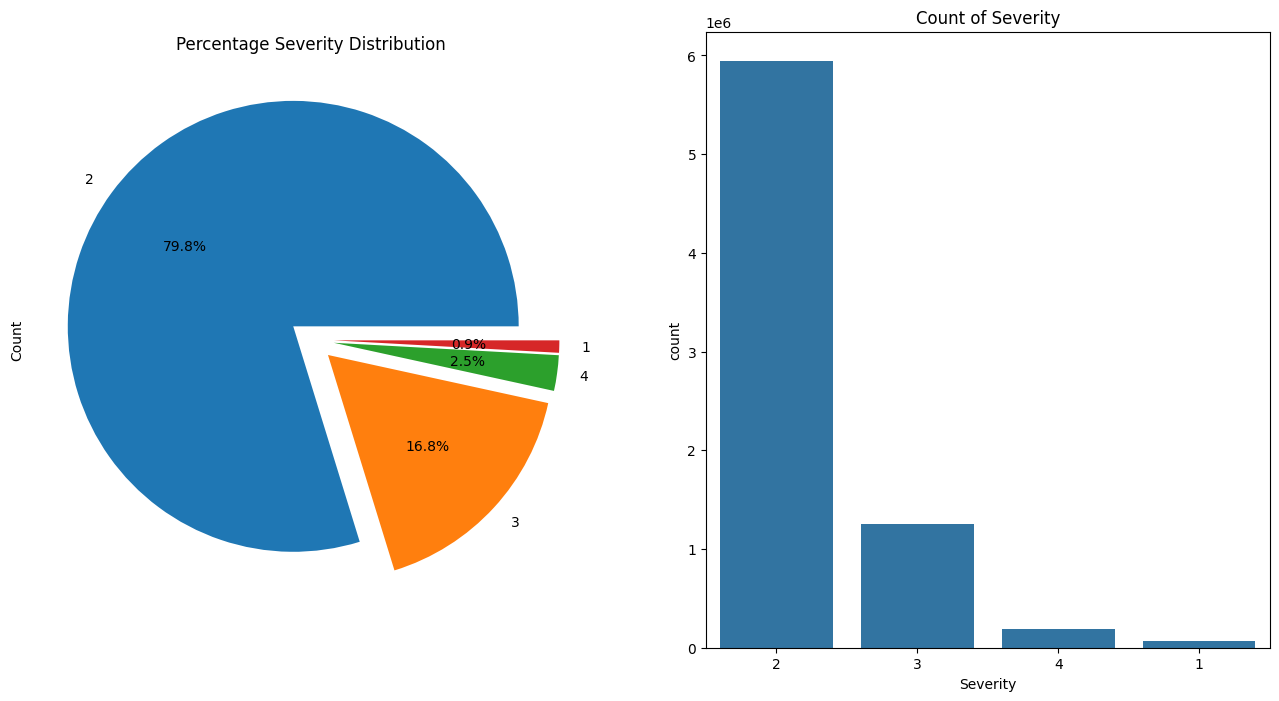
\includegraphics[width=0.5\textwidth]{graph1.png}
    \caption{\textcolor{blue}{Severity percentage}}
    \label{Fig.1}
\end{figure}

\begin{figure}[h]
    \centering
    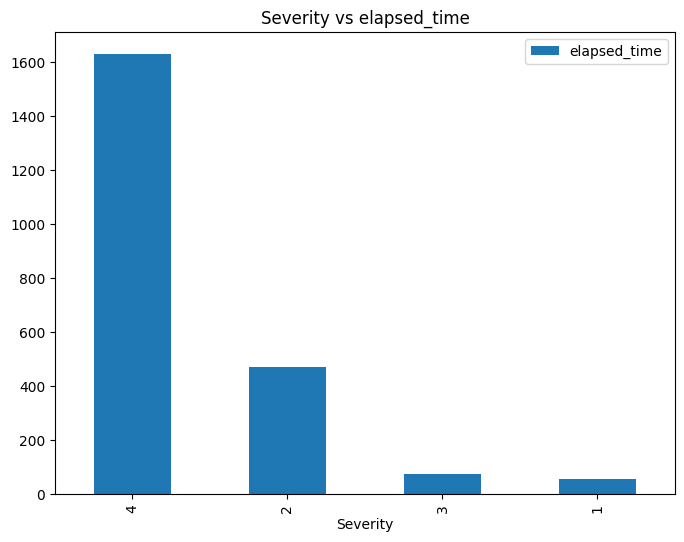
\includegraphics[width=0.5\textwidth]{graph2.png}
    \caption{\textcolor{blue}{Severity vs elapsed time}}
    \label{Fig.2}
\end{figure}

\begin{figure}[h]
    \centering
    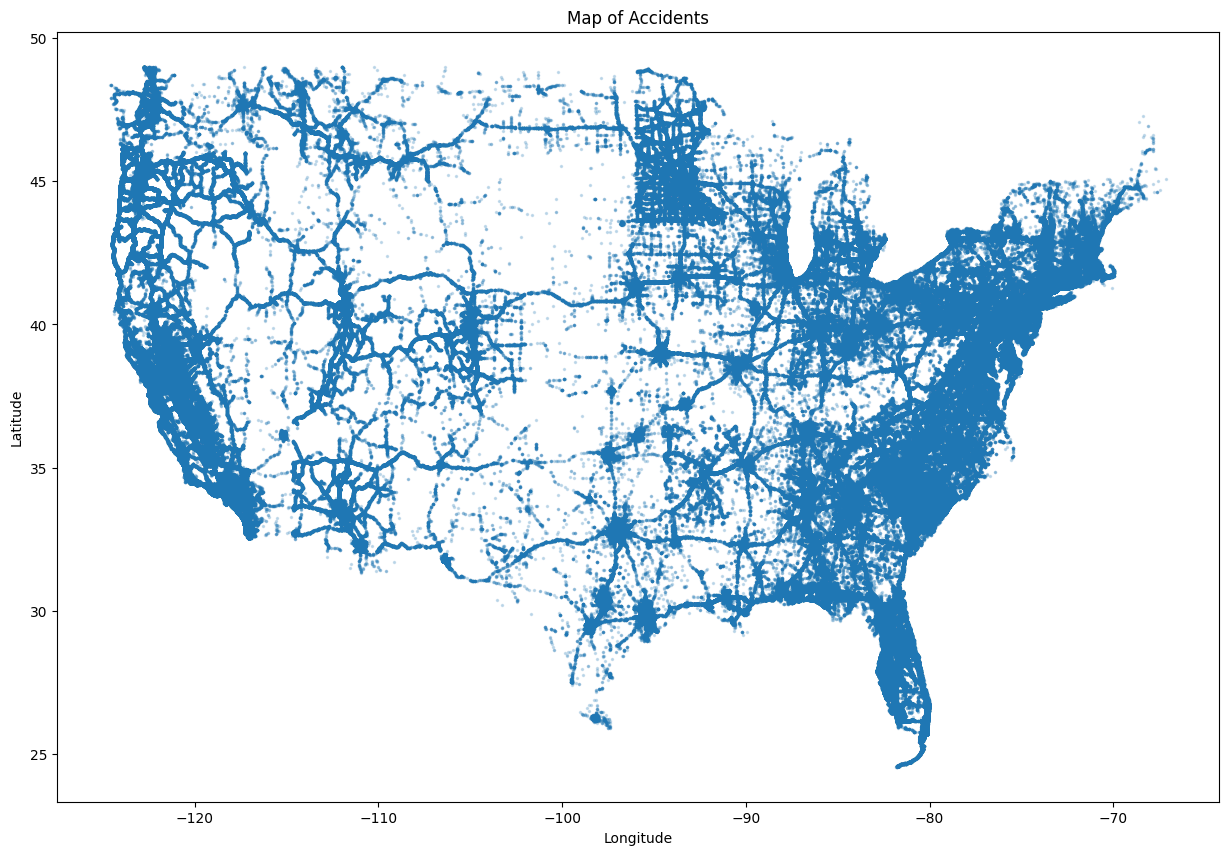
\includegraphics[width=0.5\textwidth]{graph3.png}
    \caption{\textcolor{blue}{Map of Accidents}}
    \label{Fig.3}
\end{figure}

\subsection{Normalization and Standarlization}
Initially, we conducted an outlier removal process by excluding instances where the distance column exceeded a threshold of 10. The number of rows is reduced to 7450438 after that. Subsequently, for categorical columns, we employed label encoding to convert them into numerical representations. Also, we transfromed boolean values into 0 and 1. Following this, standard scaling was applied to normalize all the columns, ensuring a consistent and comparable scale for the dataset.

\subsection{Reduce and minimize features}
We identified similarities among certain features, namely Sunrise\_Sunset, Civil\_Twilight, Nautical\_Twilight, and Astronomical\_Twilight. To streamline these features, we consolidated them into a single feature called "Twilight" using a voting mechanism. Additionally, we noted that some features exhibited a multitude of redundant classes, such as Weather\_condition with 145 distinct values and Wind\_direction with 25 different values. To address this issue, we employed feature engineering techniques, including binning or creating new features that more effectively represent the original data.

This strategic approach serves to simplify the data, leading to improved feature interpretability and enhanced model performance. Furthermore, it has the potential to mitigate overfitting in certain models. This process not only refines the dataset but also contributes to more effective and efficient modeling by reducing the complexity of features with numerous classes.
%------------------------------------------------------------------------
\section{Expected Results}
We anticipate that the experiment will identify several significant factors highly correlated with the occurrence of accidents. Building upon this knowledge, we aim to train a predictive model capable of accurately forecasting accident severity. In the future, real-time monitoring of various environmental factors will provide us with insights into the potential distribution of accident severity, aiding proactive measures and interventions.

\section{Experiment}

\subsection{Evaluation method}
In this study, we employed the f1-beta-score as our evaluation metric. Acknowledging the varying significance of precision and recall across four severity levels, we adopted distinct beta values—0.5, 1, 1, and 2 for levels 1 through 4, respectively. Following the computation of the f1-beta score for each severity level, we employed both macro and weighted averages to derive the conclusive evaluation scores. This comprehensive approach accounts for the nuanced importance of precision and recall in different severity contexts, providing a robust assessment of our model's performance.

\subsection{Experiment with different models}
To address the significant class imbalance within our dataset, we explored the efficacy of tree-based models and various boosting methods as potential solutions. In addition to the conventional Decision Tree model, we experimented with the One-vs-Rest (OnVsRest) approach. This involved training individual binary classifiers for each severity level, as opposed to a single multi-class classifier. The diverse set of candidate models was rigorously tested using our designated testing dataset, and the performance of each model was evaluated using the aforementioned metrics. This methodology allowed us to assess the models' capabilities in handling imbalanced data while providing insights into their suitability for the task at hand.

\subsection{Result}
Among the models evaluated, the ensemble method, specifically the Random Forest, outperformed the individual Decision Tree model, achieving a macro average f1-beta score of 0.65 compared to the Decision Tree's score of 0.587. Notably, the One-vs-Rest method with a Decision Tree base model exhibited a significant advantage over the original multiclass Decision Tree model. However, it is noteworthy that the One-vs-Rest method with a Random Forest base did not surpass the performance of the original Random Forest model.
In terms of boosting methods, XGBoost demonstrated superior performance among all boosting-type models, yielding a commendable score of 0.587. This performance not only surpassed the Decision Tree (0.579) but also stood out within the boosting category. Conversely, models such as SVM and a simple neural network exhibited subpar performance in addressing the challenges posed by the task at hand. These findings emphasize the effectiveness of ensemble methods and specific boosting techniques, while also highlighting the importance of choosing an appropriate base model when employing the One-vs-Rest strategy.

\begin{table}
  \centering
  \begin{tabular}{@{}lc c@{}}
    \toprule
    Method & Macro F-Beta & Weighted F-Beta \\
    \midrule
    Decision Tree & 0.579 & 0.861 \\
    Random Forest & 0.650 & 0.943 \\
    OneVsRest(decision tree) & 0.620 & 0.853 \\
    OneVsRest(random forest) & 0.642 & 0.888 \\
    SVM & 0.130 & 0.270 \\
    Neural Network & 0.476 & 0.842 \\
    AdaBoost & 0.380 & 0.799 \\
    CatBoost & 0.434 & 0.836 \\
    XGBoost & 0.587 & 0.867 \\
    \bottomrule
  \end{tabular}
  \caption{Results.}
  \label{tab:example}
\end{table}

\section{Future work}
The result shows that the highest weighted f-beta score we could get is 0.943, and the highest macro f-beta score we could get is 0.65, both results is achieved by Random Forest. Since our experiments uses default parameters for almost each models, this might indicate that the default parameters for Random Forest preform well on the dataset, but others might perform better if we tweak the parameters to better fit our datasets. In the future, we hope to tweak the parameters for each models to get the best result. Additionally, we plan to enhance prediction accuracy by incorporating external data, such as road-specific speed limits and traffic volume information. This approach aims to refine our models and further improve their performance on the given dataset.

\section{Conclusion}
In conclusion, this paper addresses the issue of traffic accidents, aiming to predict severity based on diverse environmental conditions. Despite challenges such as missing values and dataset imbalance, the systematic framework encompasses thorough data preprocessing, visualization, and feature reduction. The experiment, employing f1-beta scores, reveals the Random Forest method as the top-performing model, effectively handling the imbalanced dataset. The feature work suggests potential improvements through parameter tweaking and integration of external data, enhancing prediction accuracy. This research establishes a foundation for accident prevention, providing valuable insights for law enforcement resource optimization. Future efforts will focus on refining models and incorporating additional data sources to further enhance the predictive capabilities.

%%%%%%%%% REFERENCES
{\small
\bibliographystyle{ieee_fullname}
\bibliography{egbib.bib}
}

\end{CJK}
\end{document}
